\chapter{Implementation, Integration and Test Plan}
The application is based on three logical layers (data, logic, and presentation) that can be implemented in parallel.\\
The whole system can be tested in parallel following a bottom-up approach, this is because all the components can be developed independently and then integrated, and so the testing can be done in an incremental way to evaluate the dependencies between the subcomponents.

\section{Development plan}
Since the front-end relies on REST APIs provided by the back-end, the focus is more on the back-end development, to provide the front-end developers with the APIs needed.

\subsection{Front-end}
Even if it relies on the back-end APIs, the front-end can be developed in parallel with the back-end, since the APIs are well defined and documented.
It is sufficient to provide a mock-up of the JSON objects that will be returned by the APIs to correctly develop the front-end.

\subsection{Back-end}
Back-end development is the most important part of the project since it provides the front-end with the APIs it needs.\\
The order of development of the subcomponents is given by the dependencies between them, so the order is the following:

\begin{enumerate}
    \item \textbf{DBMS}: it is the core of the data layer, so it is the first component to be developed. It includes the implementation of the ER diagram given in Figure \ref{fig:er_diagram}
    \item \textbf{Query manager}: it is the component that provides the APIs to the logic layer that will be used to query the database. It is the second component to be developed since it relies on the DBMS and it is the only component that can access the database.
    \item \textbf{Auth manager, Notification manager}: they shall be implemented before the other subcomponents because they are used by the other subcomponents to authenticate the users and to send notifications to them. Since they are independent from each other, they can be developed in parallel.
    \item \textbf{All other subcomponents}: they can be developed in parallel since they are sufficiently independent from each other. If, for any reason, a subcomponent needs to interact with another one, it can see the other one as a black box
\end{enumerate}

\section{Integration plan}
The following section shows the order in which the subcomponents are integrated to constitute the whole system. \\
Each component must be uint tested before being integrated with the others.
The integration testing process occurs incrementally to allow for bug tracking. 
Every time a component of a dependency level is completed, it is integrated with the modules of the other levels to test the behavior of the developed subsystem. 
When the whole component is fully integrated is finally tested.\\
The order of the integration is given by the dependencies between the subcomponents, so the order is shown by the following graphs (for the sake of simplicity, the graphs show only the dependencies between the subcomponents omitting the interfaces between them):\\

The first components to integrate are the Query Manager and the DBMS since they make a connection between the application layer and the data layer. \\
\begin{figure}[H]
    \centering
    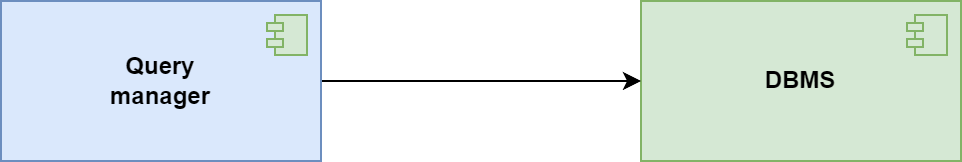
\includegraphics[width=0.6\textwidth]{images/test_plan/test-plan-1.png}
    \caption{Integration plan for the data layer}
    \label{fig:test-plan-1}
\end{figure}

The Query Manager is the only component that can access the database and nearly all the other components rely on it to query the database. \\
\begin{figure}[H]
    \centering
    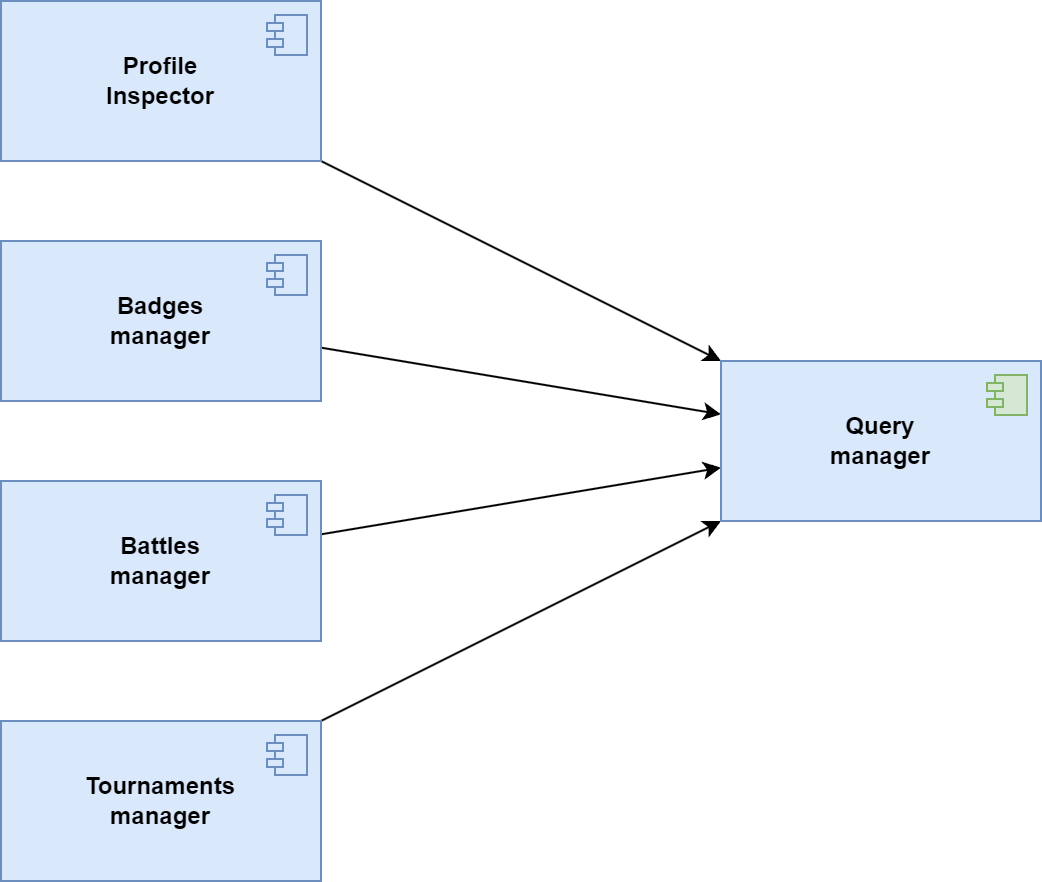
\includegraphics[width=0.6\textwidth]{images/test_plan/test-plan-3.png}
    {\color{red} Se query manager è l'unico componente che si interfaccia al DB, allora Auth Manager deve star collegato ad esso}
    \caption{Integration plan for the query manager}
    \label{fig:test-plan-3}
\end{figure}

The second component to integrate is the Auth Manager since it makes the system behave differently based on the user's permissions and so it is crucial to ensure that it works correctly before integrating other components (a concrete example is to ensure that the query to the databases are done by an authenticated user at the right level).\\
\begin{figure}[H]
    \centering
    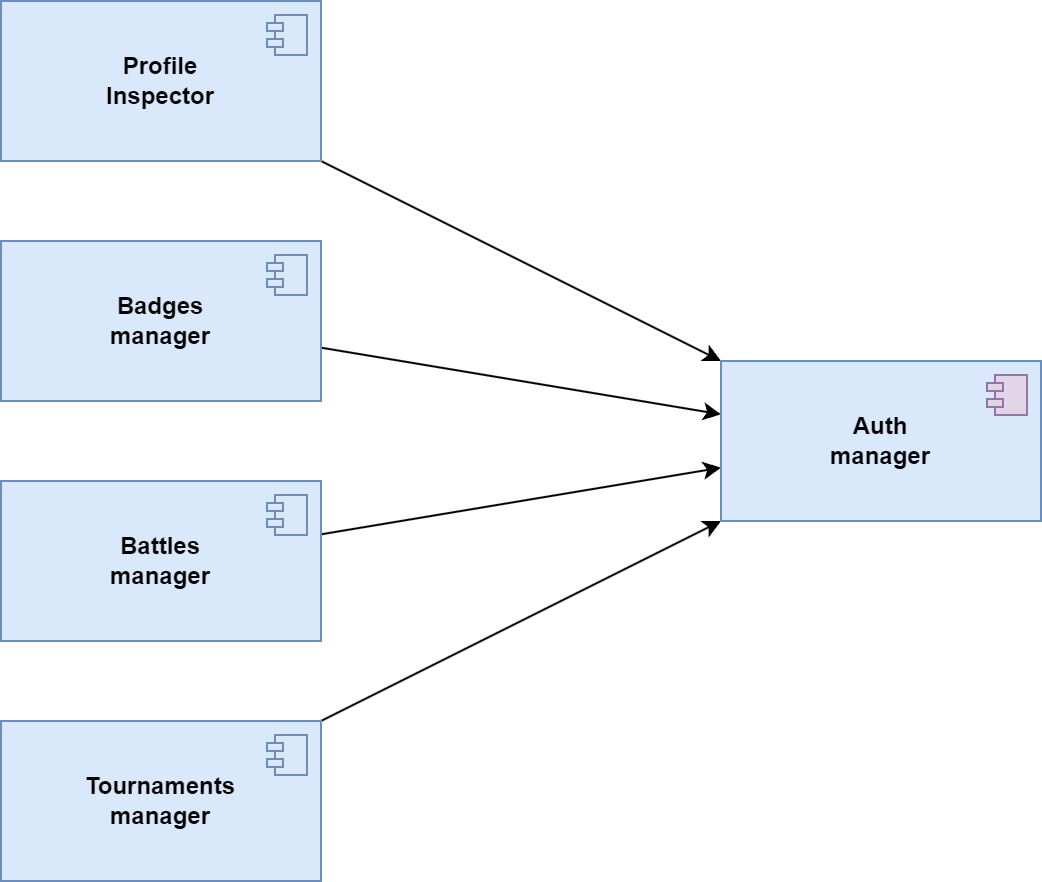
\includegraphics[width=0.6\textwidth]{images/test_plan/test-plan-2.png}
    \caption{Integration plan for the auth manager}
    \label{fig:test-plan-2}
\end{figure}

Another component to integrate is the Notification Manager, which is used to send notifications to the users. \\
It can be integrated in parallel with the Query Manager since it does not need to access the database.\\
\begin{figure}[H]
    \centering
    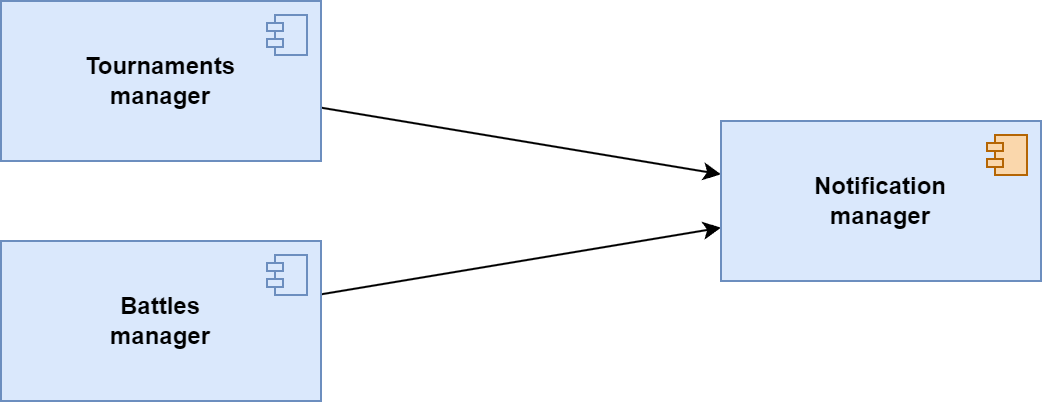
\includegraphics[width=0.6\textwidth]{images/test_plan/test-plan-4.png}
    {\color{red} Non credo si debbano mettere Profile inspector e Badges Manager}
    \caption{Integration plan for the notification manager}
    \label{fig:test-plan-4}
\end{figure}

Profile Inspector, Badge Manager, Battle Manager, and Tournament Manager are components that need to be integrated with both the Query and the Auth Manager.\\
Some of them rely on the Notification Manager as well, so they need an integration with it.\\


Finally, once all the unit tests are passed and the components are integrated, the presentation layer can be integrated with the other components and a full testing phase can be performed on the whole system.\\
\begin{figure}[H]
    \centering
    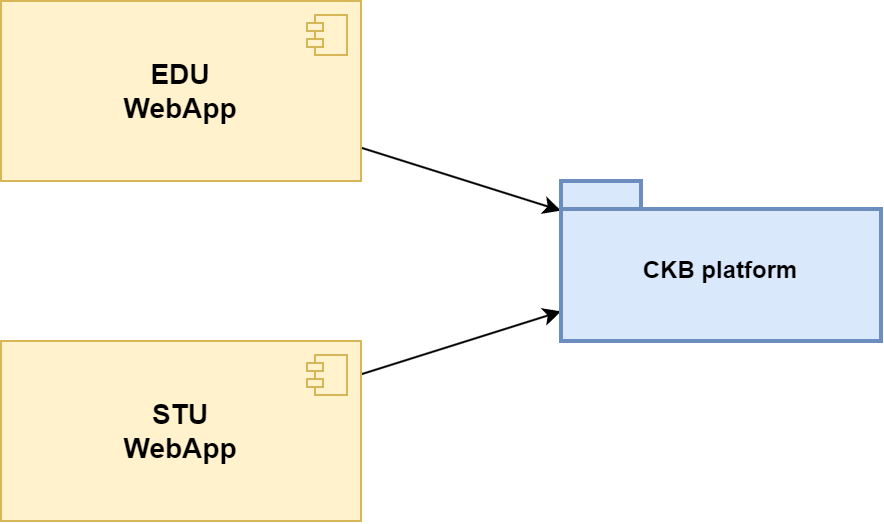
\includegraphics[width=0.6\textwidth]{images/test_plan/test-plan-5.png}
    \caption{Integration plan for the presentation layer}
    \label{fig:test-plan-5}
\end{figure}

{\color{red} Vogliamo mettere un diagramma riassuntivo di tutto l'Application server per mostrare le dipendenze?}

\section{System Testing}
The testing phase aims to verify the functional and non-functional requirements and must take place in a testing environment that is as close as possible to the production environment.\\
To ensure the minimum probability of failure of the released software, these testing performed are:
\begin{itemize}
    \item \textbf{Functional testing}: to verify that the system meets the functional requirements, in particular, the ones specified on the RASD document.
    \item \textbf{Performance testing}: to verify that the system meets the non-functional requirements, it helps to identify and eliminate performance bottlenecks affecting response time, utilization, and throughput. in particular, whether the software remains functional with increased demand and various environmental conditions.
    \item \textbf{Load testing}: to detect memory leaks, mismanagement of memory, and buffer overflows, it also identifies the maximum operating capacity of the application.
    \item \textbf{Stress testing}: to measure software robustness and error handling under heavy load conditions, it verifies stability and reliability.
\end{itemize}